\part{Analyse et Conception }
\label{part:analyse-et-conception}
\chapter{Étude préliminaire et Méthode}

Dans ce chapitre, nous allons présenter l’étude préliminaire de notre projet de
création collaborative et de partage d’arbres généalogiques, ainsi que la
méthodologie que nous allons suivre pour sa conception et son développement.
Nous commencerons par une analyse approfondie de l’existant. Nous décrirons la
situation actuelle de \firm dans le domaine de la généalogie en ligne, nous
identifierons ses limites et nous proposerons des solutions pour les surmonter.

Ensuite, nous présenterons la méthode que nous allons utiliser pour concevoir notre
plateforme. Nous mettrons l’accent sur le langage de modélisation \ac{UML} ,
ainsi que sur les différents types de diagrammes UML que nous utiliserons pour
représenter notre système de manière visuelle et structurée. Nous discuterons
également des processus de développement que nous allons adopter, notamment
le \ac{UP} et le \ac{2TUP}. Nous verrons comment ils peuvent être intégrés
à UML pour assurer une gestion efficace du projet.

Ce chapitre posera les bases nécessaires à la réalisation de notre projet en
fournissant une compréhension approfondie de son contexte et en établissant
les lignes directrices pour sa conception et son développement. En combinant
une analyse approfondie de l’existant avec une méthodologie de conception
rigoureuse, nous sommes bien placés pour créer une plateforme généalogique
collaborative et innovante qui répondra aux besoins de nos utilisateurs tout
en garantissant sa robustesse et sa pérennité.

\section{Étude de l'existant}
\subsection{Description des activités (la situation actuelle)}
Actuellement, \firm ne dispose pas d’une plateforme dédiée à la création
collaborative et au partage d’arbres généalogiques. Les activités liées à la
généalogie sont principalement effectuées de manière traditionnelle, impliquant
la collecte de documents papier, la communication verbale et l’échange de fichiers
numériques par courrier électronique ou d’autres moyens non structurés. Les
membres de la famille rencontrent souvent des difficultés pour collaborer
efficacement à la création et au partage d'arbres généalogiques en raison de
l'absence d'un outil centralisé et convivial.

\subsection{Critique de l'existant (les limites)}
Cette approche traditionnelle présente plusieurs limites. Elle rend difficile
la collaboration entre les membres de la famille, en particulier ceux qui sont
éloignés géographiquement, et ne permet pas un partage facile et sécurisé des
informations généalogiques. De plus, la préservation à long terme de l’histoire
familiale est compromise, car les documents papier peuvent se perdre ou se
détériorer avec le temps, et les fichiers numériques peuvent être dispersés et mal organisés.

\subsection{Proposition de solutions}
Pour surmonter ces défis, nous proposons les solutions suivantes :
\begin{itemize}
  \item  Utiliser des logiciels de généalogie hors ligne : cette solution implique
    l’installation de logiciels sur des ordinateurs personnels pour créer et gérer
    des arbres généalogiques. Cependant, cela peut présenter certaines limites
    en termes de collaboration et de partage, car les données sont souvent stockées
    localement et ne permettent pas une collaboration facile entre les membres de la famille.

  \item  Utiliser des sites web de généalogie : cela consiste à
    utiliser des sites web spécialisés en généalogie pour créer et partager des arbres
    généalogiques. Cette méthode est pratique, car elle permet de partager ses arbres
    avec d’autres utilisateurs. Cependant, les fonctionnalités des sites sont limitées et ne
    permettent pas toujours une collaboration efficace.

  \item Développer d’une plateforme web et mobile dédiée à la création
    collaborative et au partage d’arbres généalogiques : Cette solution propose
    de créer une plateforme personnalisée qui répond spécifiquement aux besoins de
    \firm Elle permettra aux utilisateurs de collaborer à la création d’arbres
    généalogiques, de partager facilement des informations avec leur famille et
    leurs proches, et offrira des fonctionnalités avancées, notamment la gestion
    de la confidentialité des données et des outils d’analyse.

\end{itemize}

\subsection{Choix de la solution}
Parmi les solutions présentées, nous choisissons de développer une plateforme web
et mobile dédiée à la création collaborative et au partage d’arbres généalogiques.
Elle présente la meilleure combinaison de convivialité, de fonctionnalités avancées
et de contrôle sur la confidentialité des données. En offrant une plateforme
centralisée et sécurisée, nous pouvons garantir une expérience utilisateur optimale
tout en répondant aux besoins diversifiés des utilisateurs.

En résumé, notre choix reflète notre engagement à fournir une solution
efficace et innovante pour relever les défis de \firm.

\section{Méthode}
La méthode de développement joue un rôle majeur dans la réalisation efficace
d’un projet informatique. En effet, une méthode d’analyse et de conception est
un procédé qui a pour objectif de formaliser les étapes du développement d’un
système en vue de s’assurer d’une compréhension fidèle des besoins des
utilisateurs et d’une adéquation des solutions proposées en termes de couverture
des besoins des utilisateurs. Elle fournit donc un cadre structuré pour planifier,
concevoir et mettre en œuvre des solutions logicielles répondant aux besoins
spécifiques des utilisateurs.

Il existe plusieurs types de méthodes d’analyse et de conception d’un système
d’information. Parmi celles-ci, on compte :

\begin{itemize}
  \item \textbf{Les méthodes cartésiennes ou fonctionnelles :} elles consistent
    à étudier le système par les fonctions qu'il doit assurer plutôt que par
    les données qu'il doit assurer. Le processus de conception est vu comme un
    développement linéaire.  Le domaine étudié est décomposé en sous domaines,
    eux-mêmes décomposés en sous domaines jusqu'à un niveau élémentaire ;

  \item \textbf{Les méthodes objet :} (\ac{UML} souvent associé à un \ac{UP}), elles
    sont basées sur la notion d’objet. Elle permet de modéliser les objets du
    système, leurs attributs, leurs méthodes et leurs interactions. Elle est
    largement utilisée dans l’industrie du logiciel pour concevoir et documenter
    les systèmes logiciels ;

  \item \textbf {Les méthodes agiles :} elles sont basées sur des principes
    collaboratifs et itératifs. Elles visent à fournir des solutions logicielles
    de haute qualité en s’adaptant aux besoins changeants des utilisateurs.
    Parmi les méthodes agiles les plus populaires, on compte Scrum, Kanban
    et \ac{XP}.

  \item \textbf{Les méthodes formelles :} elles s'appuient sur des techniques
    mathématiques pour spécifier, concevoir et vérifier les systèmes logiciels.
    Elles sont utilisées pour garantir la correction et la fiabilité des systèmes
    critiques.

\end{itemize}

\begin{table}[H]
  \centering
  \begin{tabular}{|p{4.5cm}|c|c|c|c|c|}
    \hline
    \textbf{\diagbox{Critères}{Méthodes}}& \textbf{Cartésiennes} & \textbf{Systémiques} & \textbf{Agiles} & \textbf{Objet} & \textbf{Formelles} \\ \hline
    Itératif & \cmark    & \cmark   & \cmark  & \cmark   & \xmark   \\ \hline
    Prise en charge de projets d’envergure   & \cmark  & \cmark    & \xmark  & \cmark   & \xmark  \\ \hline
    Incrémental                               & \xmark  & \xmark    & \cmark  & \cmark   & \xmark  \\ \hline
    Axé sur la documentation                  & \xmark  & \cmark    & \xmark  & \cmark   & \xmark  \\ \hline
    Gestion des risques                       & \xmark  & \cmark    & \cmark  & \cmark   & \xmark  \\ \hline
    Simplicité de mise en œuvre               & \xmark  & \cmark    & \cmark  & \xmark   & \xmark  \\ \hline
    Langage de modélisation                   & \xmark  & \cmark    & \xmark  & \cmark   & \cmark  \\ \hline
    Dialogue entre les intervenants du projet & \cmark  & \cmark    & \cmark  & \cmark   & \xmark  \\ \hline
    Pilotage par les cas d’utilisation        & \xmark  & \xmark    & \cmark  & \cmark   & \xmark  \\ \hline
    Axé sur le développement                  & \xmark  & \cmark    & \cmark  & \cmark   & \xmark  \\ \hline
  \end{tabular}
  \caption{Récapitulatif des méthodes }
\end{table}

Nous avons opté pour la méthode objet en raison de ses avantages. Rappelons
qu’une méthode est constituée d’un couplage entre un langage de modélisation
et un processus. Notre choix s’est arrêté sur le processus \ac{2TUP} et le
langage de modélisation UML.

\subsection{Le langage de modélisation}
Un langage de modélisation est un ensemble de conventions et de symboles utilisés pour représenter
les différents aspects d’un système complexe, comme un logiciel, un processus ou une
organisation. Selon \textcite{weilkiens2011systems}, un langage de modélisation est défini comme
\say{un langage formel utilisé pour exprimer les caractéristiques, les
comportements et les interactions d’un système sous une forme abstraite et structurée}.
Cette abstraction permet aux développeurs et aux ingénieurs de
communiquer efficacement et de collaborer sur la conception, la modélisation et l’analyse des
systèmes complexes. Ainsi, l’importance d'un langage de modélisation réside dans sa capacité à fournir une représentation
visuelle claire et concise des différents éléments d'un système, ainsi que de leurs interactions.
Il existe deux types de langage de modélisation : les langages de modélisation graphique
et les langages de modélisation textuelle.

Les langages de modélisation graphique utilisent des techniques de diagramme
avec des symboles associés à des noms qui représentent les concepts, des lignes
qui connectent les symboles et qui représentent les relations et d’autres
annotations graphiques pour représenter les contraintes.

Les langages de modélisation textuelle utilisent typiquement des mots-clés
standardisés accompagnés de paramètres pour rendre les expressions interprétables
par les ordinateurs.

\subsubsection{Présentation d'UML}
\ac{UML} est un langage de modélisation largement utilisé dans l’industrie
du logiciel pour la conception, la documentation et la communication des systèmes logiciels.
Initialement créé par Grady Booch, Ivar Jacobson et James Rumbaugh, UML est devenu une norme
de facto pour la modélisation des systèmes orientés objet.

UML propose un ensemble de conventions et de diagrammes qui permettent de
représenter visuellement les différents aspects d’un système logiciel. Ces
diagrammes peuvent être utilisés pour décrire la structure statique d’un système,
ses comportements dynamiques, ses interactions avec d’autres systèmes, et bien
plus encore. En utilisant UML, les développeurs et les ingénieurs peuvent
collaborer efficacement, communiquer clairement et documenter de manière précise
les spécifications d’un projet logiciel.

Selon \textcite{fowler2003uml}, UML peut être considéré comme le
\say{langage de modélisation standard} pour exprimer la conception d’un système
logiciel. En fournissant un cadre formel et structuré pour la modélisation des
systèmes informatiques, UML permet aux parties prenantes du projet de mieux
comprendre les besoins, les exigences et les contraintes du système. Cela facilite
la prise de décision et la gestion des risques tout au long du cycle de vie du projet.

\subsubsection{Les types de diagrammes d'UML}
UML propose une variété de diagrammes qui permettent de représenter différents
aspects d'un système logiciel. Ces diagrammes sont catégorisés en deux grandes
classes : les diagrammes structurels et les diagrammes comportementaux.

Les diagrammes structurels sont utilisés pour décrire la structure statique
d’un système logiciel, c’est-à-dire ses composants, leurs relations et leur
organisation. Parmi les principaux diagrammes structurels d’UML, on compte :

\begin{itemize}

  \item Le diagramme de classe : il représente les classes du système, ainsi que leurs
    attributs, méthodes et relations.

  \item Le diagramme d’objet : il montre des instances spécifiques de classes
    et les liens entre elles.

  \item Le diagramme de composants : il décrit les composants physiques du
    système et leurs dépendances.

  \item Le diagramme de déploiement : il représente la configuration matérielle
    sur laquelle le système est déployé.

\end{itemize}


Quant aux diagrammes comportementaux, ils se concentrent sur le comportement
dynamique du système, c’est-à-dire sur la manière dont il réagit et interagit
avec son environnement. Les principaux diagrammes comportementaux d’UML sont
les suivants :

\begin{itemize}

  \item  Le diagramme de cas d’utilisation : il décrit les interactions entre
    le système et ses utilisateurs, en mettant l’accent sur les fonctionnalités
    offertes par le système.

  \item Le diagramme de séquence : il montre la séquence des messages échangés
    entre les objets du système au cours d’un scénario d’exécution.

  \item Le diagramme d’état : il représente les différents états possibles d’un
    objet et les transitions entre ces états.

  \item Le diagramme d’activité : qui décrit le flux de contrôle entre les
    différentes activités du système.

\end{itemize}

Il est important de souligner que: UML n’est pas une méthode ;
l’utilisation des diagrammes est donc laissée à l’appréciation de chacun.
Le diagramme de classes est généralement considéré comme l’élément central d’UML.

\subsection{Processus de développement}
Dans le domaine du génie logiciel, le processus de développement est un ensemble
d’activités et d’étapes requises pour la création d’un système logiciel.
Parmi les nombreuses approches disponibles, deux méthodes largement utilisées
sont l’Unified Process (\ac{UP}) et le Two-Tiered Unified Process (\ac{2TUP}).

\subsubsection{Présentation du UP}
L’UP est un processus itératif et incrémental de développement logiciel. Il est
basé sur le principe de gestion de projet itératif et itératif-incrémental, dans
lequel le développement est divisé en plusieurs phases, chacune produisant des
livrables spécifiques. Ces phases comprennent l’élaboration, la construction,
la transition, et la production de divers artefacts tels que des spécifications,
des modèles UML, et des versions de logiciel partielles ou complètes. L’UP se
distingue par son adaptabilité, sa flexibilité et sa focalisation sur la qualité du produit final.

\subsubsection{Présentation du 2TUP}
Le 2TUP est une adaptation du UP conçue pour être plus flexible et adaptable aux
projets de taille moyenne ou grande. Il se compose de deux branches : la branche
fonctionnelle et la branche technique, ainsi qu’une phase de réalisation.
La branche fonctionnelle permet de capturer les besoins, les spécifications et
l’analyse. La branche technique permet la capture des besoins techniques, l’architecture
logicielle et applicative ainsi que les frameworks techniques. Quant à la phase
de réalisation, elle inclut la conception, le codage, les tests et la recette
ou le déploiement.

Cette approche permet une personnalisation accrue du processus de développement en
fonction des particularités et des contraintes du projet.

\newpage
\begin{figure}[H]
  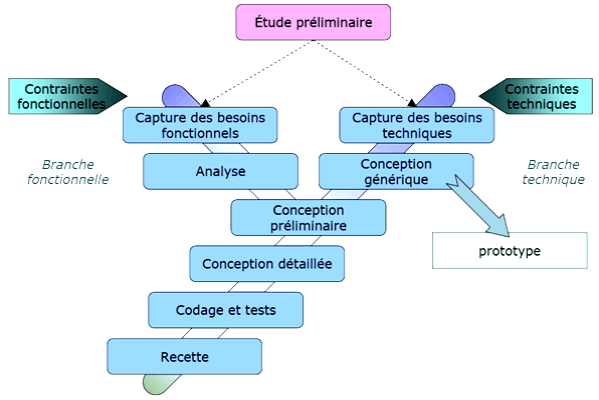
\includegraphics{./figure/illustrationDeveloppementEnY.png}
  \caption{Illustration du processus de développement en Y}
\end{figure}



\subsubsection{2TUP et UML}
L’utilisation de UML est étroitement liée au 2TUP. Les différents types de
diagrammes UML (diagramme de cas d’utilisation, de classes, de séquence et d’état)
sont largement utilisés tout au long du processus de développement pour modéliser
et documenter les besoins, les architectures, les interactions et les comportements
du système logiciel en cours de développement. UML fournit un langage visuel
standard et universellement accepté pour la représentation des systèmes logiciels.
Cela facilite la communication et la collaboration entre les membres de l’équipe
de développement et les
parties prenantes du projet.


\chapter{Analyse et conception}
Ce chapitre se concentre sur l’analyse approfondie des besoins de la plateforme
web et mobile pour la création collaborative et le partage d’arbres généalogiques
à \firm. Il présente également la conception de cette plateforme. L’analyse
approfondie des besoins est une étape importante dans le processus de développement,
car elle permet de définir clairement les fonctionnalités et les exigences
techniques nécessaires à la réalisation du projet. La conception, quant à elle,
vise à traduire ces besoins en solutions techniques efficaces et robustes.
Ce chapitre présentera donc en détail les besoins fonctionnels et techniques
identifiés lors de l’analyse, donnant ainsi les bases solides pour la conception de la plateforme.


\section{Analyse du besoin}
L'analyse du besoin vise à comprendre en profondeur les attentes et les exigences
des utilisateurs ainsi que les contraintes techniques et fonctionnelles qui
guideront le développement de la plateforme. Cette analyse repose sur une
étude approfondie des besoins fonctionnels et techniques.

\subsection{Besoins fonctionnels}
Les besoins fonctionnels définissent les fonctionnalités et les services que la
plateforme doit fournir à ses utilisateurs. Ils sont étroitement liés aux
objectifs et aux cas d’usage du système. Ces besoins incluent :

\begin{itemize}

  \item Création et gestion d’arbres généalogiques : les utilisateurs enregistrés
    peuvent créer, modifier et supprimer des arbres généalogiques et gérer les
    informations sur leurs proches;

  \item Consultation des arbres existants : les utilisateurs doivent pouvoir
    consulter les arbres généalogiques disponibles, y compris les détails sur
    les membres de leur famille;

  \item Recherche de membres de la famille : les utilisateurs doivent pouvoir
    trouver des personnes dans les arbres généalogiques existants sans avoir à
    créer de compte;

  \item Collaboration entre utilisateurs sur le même arbre : les utilisateurs
    enregistrés doivent pouvoir collaborer à la création et à la gestion d’un
    arbre généalogique, en y ajoutant, modifiant ou supprimant des informations
    sur les membres de la famille;

  \item Gestion des droits d’accès et de confidentialité : les utilisateurs doivent
    pouvoir déterminer qui aura accès aux arbres généalogiques qu’ils ont créés et
    gérés. Ils peuvent ainsi contrôler qui peut consulter, modifier ou contribuer
    aux informations contenues dans l’arbre;

  \item Partage et diffusion des arbres : les utilisateurs doivent pouvoir partager
    leurs arbres généalogiques avec leur famille et leurs proches.
    Ceux-ci auront alors accès à des versions consultables et visualisables.

\end{itemize}

\subsection{Besoins techniques}
Les besoins techniques décrivent les contraintes et les exigences liées à l’infrastructure
et aux technologies utilisées pour développer la plateforme. Cela inclut :

\begin{itemize}
  \item \textbf{Le choix des technologies de développement :} les langages de
    programmation, les frameworks et les outils qui seront utilisés pour créer
    la plateforme. Dans notre cas, nous utilisons :
    \begin{itemize}
      \item Langage de programmation : TypeScript (web et mobile)
      \item Frameworks : Next.js (web), Expo (mobile)
    \end{itemize}

  \item \textbf{La gestion des données :} la manière dont les informations sur les
    arbres généalogiques et les membres de la famille seront stockées, gérées
    et sécurisées. Les données sont stockées dans une base de données
    PostgreSQL. Prisma est utilisé pour gérer les opérations de base de
    données, assurant l'intégrité et la sécurité des données grâce à des
    schémas stricts et des migrations contrôlées. Et Docker est utilisé pour
    créer un conteneurs pour le \ac{SGBD};

  \item \textbf{L’interface utilisateur :} la conception de l’interface utilisateur
    pour garantir une expérience utilisateur intuitive et conviviale.
    Next.js est utilisé pour le rendu côté serveur et les pages réactives,
    assurant une performance élevée et une expérience utilisateur fluide;

  \item \textbf{La compatibilité et la sécurité :} la compatibilité avec les navigateurs
    web et les appareils mobiles, la sécurité des données, la scalabilité pour
    gérer un grand nombre d’utilisateurs, ainsi que l’interopérabilité avec
    d’autres systèmes et services existants. Les pages et composants sont
    testés pour être compatibles avec les principaux navigateurs
    (Chrome, Firefox, Safari) et optimisés pour les appareils mobiles. Docker
    permet de facilement faire évoluer l'application pour gérer une augmentation du
    nombre d'utilisateurs. Les mesures de sécurité incluent l'utilisation de
    HTTPS, la gestion des sessions sécurisées, et des pratiques de développement
    sécurisées pour éviter les vulnérabilités courantes;

  \item \textbf{La gestion des erreurs :} la gestion des erreurs et des exceptions
    pour garantir la fiabilité et la robustesse de la plateforme. Les erreurs
    sont gérées de manière élégante et informative pour les utilisateurs, tout
    en étant enregistrées et surveillées pour permettre une résolution rapide
    des problèmes.

\end{itemize}

\section{Conception du système}
Dans cette section, nous aborderons les spécifications fonctionnelles du
système. Nous décrirons les acteurs impliqués, les cas d’utilisation identifiés,
ainsi que les relations et la classification de ces cas d’utilisation.

\subsection{Spécifications fonctionnelles}
Les spécifications fonctionnelles décrivent les fonctionnalités et les interactions
du système avec ses utilisateurs. Elles fournissent une vue détaillée des
besoins opérationnels du système.

\subsubsection{Identification des acteurs}
Les acteurs sont les entités externes qui interagissent avec le système.
Dans notre plateforme de création collaborative et de partage d'arbres
généalogiques à Mazala-Firm, les acteurs identifiés comprennent :

\begin{itemize}
  \item les membres;

  \item les créateurs d'arbre;

  \item les administrateurs;

  \item et les visiteurs.

\end{itemize}

\subsubsection{Diagramme de contexte statique}
Le diagramme de contexte statique représente graphiquement les acteurs et leurs
relations avec le système. Il fournit une vue d’ensemble claire des interactions
entre les différentes entités impliquées dans notre plateforme de création
collaborative et de partage d’arbres généalogiques. Ce diagramme met en évidence
les liens essentiels entre les utilisateurs inscrits, les administrateurs du
système et les visiteurs non enregistrés, ce qui illustre la dynamique de
notre écosystème numérique.

\begin{figure}[H]
  \centering
  \begin{tikzpicture}[node distance=2cm, every node/.style={inner sep=3pt}]
    \node (system) [draw, rectangle, minimum width=2.5cm, text width=2cm, align=center] {: Système};
    \node (utilisateurs) [above left=of system] {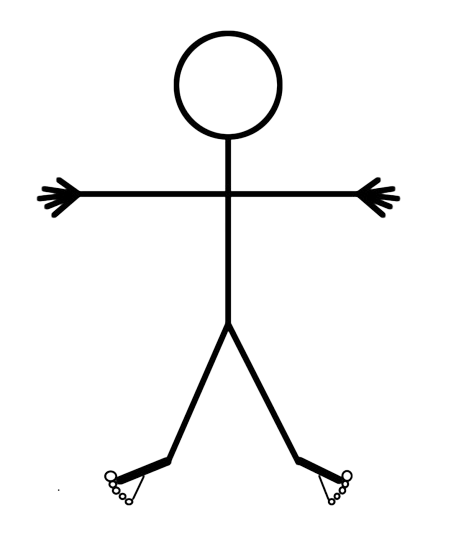
\includegraphics[width=1cm]{images/stickman.png}};
    \node (admins) [above right=of system] {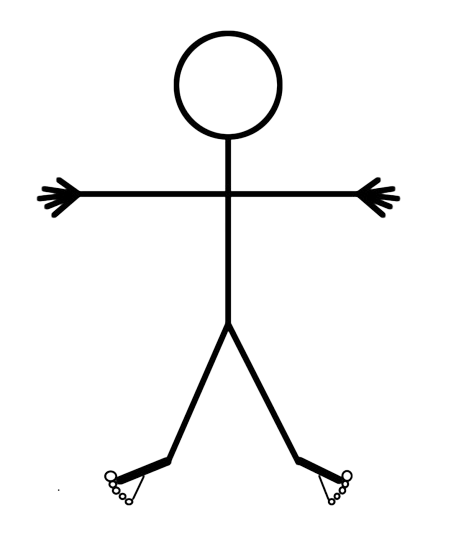
\includegraphics[width=1cm]{images/stickman.png}};
    \node (visiteurs) [below left=of system] {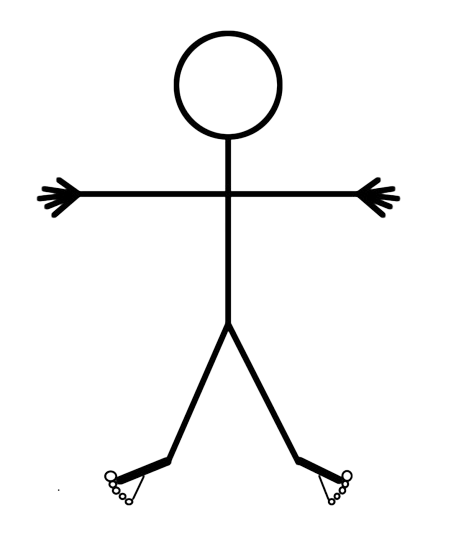
\includegraphics[width=1cm]{images/stickman.png}};
    \node (owner) [below right=of system] {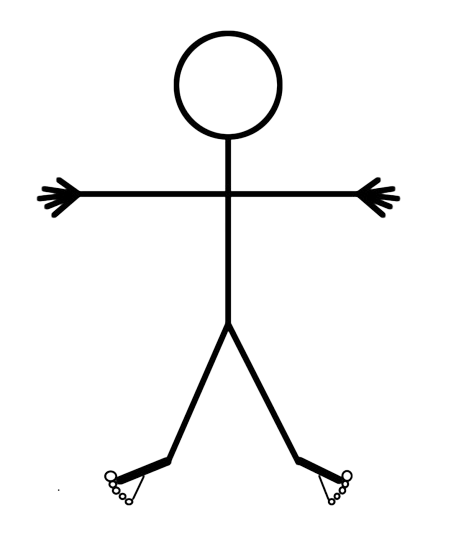
\includegraphics[width=1cm]{images/stickman.png}};

    \draw[->] (utilisateurs) -- node[anchor=south] {1..*} (system);
    \draw[->] (owner) -- node[anchor=south] {1..*} (system);
    \draw[->] (admins) -- node[anchor=east] {1..*} (system);
    \draw[->] (visiteurs) -- node[anchor=east] {1..*} (system);

    \node[below=0.3cm of utilisateurs] {Membre};
    \node[below=0.3cm of owner] {Créateur d'arbre};
    \node[below=0.3cm of admins] {Administrateur};
    \node[below=0.3cm of visiteurs] {Visiteurs};
  \end{tikzpicture}
  \caption{Diagramme de contexte statique}
\end{figure}


\subsubsection{Identification des cas d'utilisation}
Les cas d'utilisation décrivent les interactions entre les acteurs et le
système afin d'atteindre des objectifs spécifiques. Pour notre système, on retrouve :

\begin{itemize}
  \item Créer un compte
  \item S'authentifier
  \item Gérer un arbre généalogique;
  \item Gérer des membres;
  \item Consulter un arbre généalogique;
  \item Rechercher des membres de la famille;
  \item Accorder des droits d'accès;
  \item Partager un arbre généalogique;
  \item Administrer le système.
\end{itemize}

\subsubsection{Relation entre les cas d'utilisation (Use case)}
Pour affiner la représentation des interactions entre les différents cas
d’utilisation de notre système, nous utilisons les relations standardisées
définies par UML. Ces relations permettent de mieux comprendre les liens entre
les différentes fonctionnalités du système. Voici comment elles s’appliquent
dans notre contexte :

\begin{itemize}
  \item Inclusion (\say{include}) : cette relation est utilisée lorsqu’un cas
    d’utilisation de base incorpore explicitement un autre cas d’utilisation,
    de manière obligatoire. Dans notre système, nous pourrions par exemple
    inclure le cas d’utilisation \say {Modifier les informations des membres}
    dans le cas d’utilisation \say{Gérer des membres}, car la modification des
    informations des membres fait partie intégrante de la gestion des membres.
    De même, le cas d'utilisation \say{S'authentifier} est inclus dans tous
    les cas d'utilisation des membres et de l'administrateur, car ils doivent
    être authentifiés avant de réaliser toute autre action.

  \item Extension (\say{extend}) : cette relation est utilisée lorsqu’une
    utilisation de base incorpore implicitement un autre cas d’utilisation, de
    façon optionnelle. Par exemple, le cas d’utilisation \say{Partager un arbre généalogique}
    peut être étendu par le cas d’utilisation \say{Accorder des droits d’accès et de confidentialité}.
    Ainsi, lorsqu’un utilisateur souhaite partager un arbre généalogique, il a
    également la possibilité d’accorder des droits d’accès spécifiques à
    certains membres de sa famille.

  \item Généralisation/spécialisation : cette relation sert à décrire un lien
    du genre \say{est un} entre différents cas d’utilisation. Dans notre système,
    on peut trouver une généralisation entre les cas d’utilisation \say {Gérer un
    arbre généalogique} et \say{Gérer des membres}, puisque gérer un arbre
    généalogique inclut aussi la gestion des membres qui en font partie. Les
    fonctionnalités de gestion des membres peuvent donc être considérées comme
    une spécialisation du cas d’utilisation de gestion d’un arbre généalogique.
\end{itemize}

\newpage
\begin{figure}
  \begin{tikzpicture}

% Actors
\umlactor[x=-3, y=5]{Visiteur}
\umlactor[x=-3, y=2]{Membre}
\umlactor[x=-3, y=-1]{Créateur d'arbre}
\umlactor[x=-3, y=-3]{Administrateur}

% Use Cases
\begin{umlsystem}[x=0, y=0, fill=white]{Système}
  \umlusecase[x=3, y=5]{Créer compte}
  \umlusecase[x=3, y=4]{Consulter arbre}
  \umlusecase[x=3, y=3]{Rechercher membres}
  \umlusecase[x=3, y=2]{Gérer membres}
  \umlusecase[x=3, y=1]{Partager arbre}
  \umlusecase[x=3, y=0]{Accorder droits}
  \umlusecase[x=3, y=-1]{Gérer arbre}
  \umlusecase[x=3, y=-2]{Administrer}
  \umlusecase[x=10, y=1]{S'authentifier}
\end{umlsystem}

% Associations
\umlassoc{Visiteur}{usecase-1}
\umlassoc{Visiteur}{usecase-2}
\umlassoc{Visiteur}{usecase-3}
\umlassoc{Membre}{usecase-4}
\umlassoc{Membre}{usecase-5}
\umlassoc{Créateur d'arbre}{usecase-6}
\umlassoc{Créateur d'arbre}{usecase-7}
\umlassoc{Administrateur}{usecase-8}

% Relationships
\umlinclude{usecase-4}{usecase-9}
\umlinclude{usecase-5}{usecase-9}
\umlinclude{usecase-6}{usecase-9}
\umlinclude{usecase-7}{usecase-9}
\umlinclude{usecase-8}{usecase-9}

\umlaggreg{Visiteur}{Membre}
\umlaggreg{Membre}{Créateur d'arbre}

\end{tikzpicture}
  \caption{Diagramme de cas d'utilisation}
\end{figure}

\subsubsection{Classification des cas d'utilisation (priorités, risques et itérations)}
Dans cette section, nous classons les cas d’utilisation identifiés selon leur
priorité, leur niveau de risque et leur inclusion dans les itérations du
développement. Cette classification servira à guider la planification et
l’exécution du projet en mettant en évidence les fonctionnalités les plus
importantes, les risques potentiels à surveiller et les étapes itératives du
développement.

% |m{4cm}|m{11cm}|
\begin{table}[H]
  \centering
  \begin{tabular}{|l|l|l|c|}
    \hline
    \textbf{Cas d'utilisation} & \textbf{Priorité} & \textbf{Risque} & \textbf{Itération} \\ \hline
    S'authentifier & Forte & Moyen & 1 \\ \hline
    Géer un compte & Moyenne & Moyen & 1 \\ \hline
    Gérer un arbre généalogique & Forte & Moyen & 1 \\ \hline
    Gérer des membres & Forte & Moyen & 1 \\ \hline
    Consulter un arbre généalogique & Forte & Faible & 1 \\ \hline
    Rechercher des membres de la famille & Moyenne & Moyen & 2 \\ \hline
    Partager un arbre généalogique & Forte & Élevé & 2 \\ \hline
    Accorder des droits d’accès  & Moyenne & Élevé & 3 \\ \hline
    Administrer le système & Moyenne & Élevé & 3 \\ \hline
  \end{tabular}
  \caption{Classification des cas d'utilisation}
\end{table}


Dans le tableau ci-dessus, chaque cas d’utilisation est évalué selon trois critères principaux :

\begin{itemize}

  \item Priorité : indique l’importance relative du cas d’utilisation pour
    l’achèvement du projet. Les priorités peuvent être classées comme forte, moyennes ou basses.

  \item Risque : évalue le niveau de risque associé à la mise en œuvre du cas
    d’utilisation. Les risques peuvent être classés comme faibles, moyens ou élevés.

  \item Itération : indique dans quelle itération du développement le cas
    d’utilisation sera implémenté. Les itérations peuvent être numérotées séquentiellement.

\end{itemize}

Cette classification constituera un outil précieux pour la planification et la
gestion du projet. Elle permettra une allocation efficace des ressources et
une identification proactive des risques potentiels.

\subsection{Spécification détaillée }
Dans cette section, nous fournissons une spécification détaillée des cas
d’utilisation identifiés. Nous décrivons les interactions entre les acteurs et
le système, ainsi que les flux d’événements associés.

\subsubsection{Description textuelle d'un cas d'utilisation}
\textbf{Cas d’utilisation :} Gérer un arbre généalogique

\textbf{Acteur :} Membre

\textbf{Autres acteurs :} Système

\textbf{Date :} 15/04/2024

\textbf{Version :} 1.3

\textbf{Description :} Ce cas d’utilisation permet à le membre de créer,
de modifier, de visualiser et de supprimer des arbres généalogiques.

\textbf{Préconditions :} Le membre est authentifié et peut accéder à la
fonctionnalité de gestion des arbres généalogiques.

\textbf{Séquencement des événements}

Le cas d’utilisation commence lorsque le membre se connecte à la plateforme
et desire gérer un arbre généalogique.

\textbf{Scénario nominal :}

\begin{enumerate}

  \item  Le membre se connecte à l’application.

  \item Le système affiche alors une barre de navigation latérale comportant un
    bouton \say{Créer un arbre} ainsi qu’une liste d’arbres généalogiques déjà
    existants chez ce membre.

  \item Le membre peut ensuite sélectionner parmi les options suivantes :
    \begin{itemize}
      \item Créer un nouvel arbre généalogique;
      \item Modifier un arbre généalogique existant;
      \item Consulter un arbre généalogique existant;
      \item Supprimer un arbre généalogique existant;
      \item Visualiser un arbre généalogique existant.
    \end{itemize}

  \item Si le membre décide de créer un nouvel arbre généalogique :
    \begin{enumerate}
      \item il doit cliquer sur le bouton \say{Créer un nouvel arbre};
      \item le système affiche une fenêtre où il devra entrer un nom et un type(publique, privé)
        pour son nouvel arbre généalogique;
      \item le membre valide ses informations;
      \item le système crée alors un nouvel arbre généalogique et l’affiche dans la liste des arbres
        généalogiques du membre.
    \end{enumerate}

  \item  Si le membre décide de modifier un arbre généalogique existant :
    \begin{enumerate}
      \item il sélectionne l’arbre généalogique dans la barre de navigation latérale.;
      \item le système affiche alors les détails de l’arbre généalogique sélectionné;
      \item le membre effectue les modifications nécessaires (ajouts,
        suppressions, modifications de membres ou de relations) ou les
        informations de l’arbre généalogique;

        \subitem Pour ajouter un membre :

          \begin{itemize}
            \item le membre clique sur l’option \say{Ajouter un membre};
            \item le e système présente un formulaire qui demande des
              renseignements au sujet du nouveau membre (son nom, sa date de
              naissance, ses relations, etc.);
            \item le membre remplit les champs requis et valide son entrée;
            \item le système ajoute le nouveau membre à l’arbre généalogique;
          \end{itemize}

        \subitem Pour modifier les informations de l’arbre généalogique :

          \begin{itemize}
            \item le membre clique sur l’option \say{Modifier les informations};
            \item le système affiche un formulaire de modification des informations de l’arbre généalogique;
            \item le membre effectue les modifications nécessaires et valide ses changements;
            \item le système enregistre les modifications apportées à l’arbre généalogique.
          \end{itemize}

      \item le système sauvegarde toutes les modifications apportées à l’arbre généalogique.
    \end{enumerate}

  \item Si le membre souhaite consulter, un arbre généalogique existant :
    \begin{enumerate}
      \item il sélectionne l’arbre généalogique dans la barre de navigation latérale;
      \item le système affiche alors l’arbre généalogique sélectionné avec les
        informations sur ses membres et leurs liens.
    \end{enumerate}

  \item Si le membre souhaite supprimer un arbre généalogique existant :
    \begin{enumerate}
      \item il sélectionne l’arbre généalogique dans la barre de navigation latérale;
      \item le système demande une confirmation avant de procéder à la
        suppression définitive de l’arbre généalogique;
      \item si le membre accepte, le système efface l’arbre généalogique
        ainsi que toutes les données connexes de la liste dans la barre de
        navigation latérale.
    \end{enumerate}

\end{enumerate}

\textbf{Scénarios alternatifs :}
% \subsubsection*{Scénarios alternatifs}

\begin{enumerate}
    \item \textbf{Scénario alternatif pour la création d'un arbre généalogique :}
    \begin{itemize}
        \item \textbf{Étape 4a :} Le membre tente de créer un arbre
          généalogique mais ne saisit pas un nom valide ou ne choisit pas un type.
        \begin{itemize}
            \item le système affiche un message d'erreur demandant de saisir
              un nom valide ou de choisir un type;
        \end{itemize}
        Le scénario reprend à l'étape 4c.
    \end{itemize}

    \item \textbf{Scénario alternatif pour la modification d'un arbre généalogique :}
    \begin{itemize}
        \item \textbf{Étape 5a :} Le membre laisse des champs obligatoires vides.
        \begin{itemize}
            \item le système affiche un message d'erreur demandant de compléter les champs obligatoires;
        \end{itemize}
        Le scénario reprend à l'étape 5c.
    \end{itemize}

  \item \textbf{Scénario alternatif pour la visualisation d'un arbre généalogique :}
    \begin{itemize}
      \item \textbf{Étape 6a :} Le membre tente de visualiser un arbre
        généalogique mais celui-ci contient des erreurs de données (ex. : relations incorrectes).
        \begin{itemize}
          \item le système affiche un message d'erreur et propose des options de correction.
          \item le membre corrige les erreurs.
        \end{itemize}
        Le scénario reprend à l'étape 6a.
    \end{itemize}

    \item \textbf{Scénario alternatif pour la suppression d'un arbre généalogique :}
    \begin{itemize}
        \item \textbf{Étape 7a :} Le membre sélectionne un arbre généalogique à supprimer mais change d'avis et annule l'opération.
        \begin{itemize}
            \item Le système annule l'opération de suppression et revient à la liste des arbres généalogiques.
        \end{itemize}
    \end{itemize}


\end{enumerate}

\textbf{Scénario d'exception :}
\begin{enumerate}
  \item Si, à l’étape 3, le membre ferme la barre de navigation latérale
    ,le scénario principal est interrompu.

  \item Si le membre essaie de supprimer un arbre généalogique sans avoir
    obtenu de confirmation, le système annule
\end{enumerate}

\textbf{Postconditions :} Les modifications apportées à l'arbre généalogique
sont enregistrées dans le système.

Cette description textuelle fournit une vue détaillée des étapes et des
interactions impliquées dans le cas d’utilisation \say{Gérer un arbre généalogique}.
\\

\textbf{Cas d’utilisation :} Accorder des droits d’accès

\textbf{Acteur :} Créateur d'arbre

\textbf{Autres acteurs :} Système

\textbf{Date :} 15/04/2024

\textbf{Version :} 1.0


\textbf{Description :} Ce cas d’utilisation permet au créateur d'arbre d'accorder,
de modifier, et de révoquer des droits d'accès aux  membres pour
les arbres généalogiques.

\textbf{Préconditions :} Le créateur d'arbre est authentifié et possède les droits
nécessaires pour gérer les accès aux arbres généalogiques.


\textbf{Séquencement des événements}

Le cas d’utilisation commence lorsque le créateur d'arbre se connecte à la
plateforme et désire gérer les droits d'accès à un arbre généalogique.

\textbf{Scénario nominal :}

\begin{enumerate}

  \item  Le créateur d'arbre se connecte à l’application.

  \item Le système affiche une barre de navigation latérale comportant un
    bouton \say{Gérer les droits d’accès} ainsi qu’une liste d’arbres
    généalogiques pour lesquels il a des droits de gestion.

  \item Le créateur d'arbre sélectionne l'arbre généalogique pour lequel il souhaite
    gérer les droits d'accès.

  \item Le système affiche une interface permettant de voir les membres
    actuels et leurs niveaux d'accès.

  \item Le créateur d'arbre peut ensuite sélectionner parmi les options suivantes :
    \begin{itemize}
      \item Ajouter des droits d'accès pour un nouveau membre;
      \item Modifier les droits d'accès pour un membre existant;
      \item Révoquer les droits d'accès pour un membre existant.
    \end{itemize}

  \item Si le créateur d'arbre décide d'ajouter des droits d'accès pour un nouveau membre :
    \begin{enumerate}
      \item il doit cliquer sur le bouton \say{Ajouter un membre};
      \item le système affiche une fenêtre où il devra entrer l'identifiant du
        membre et choisir le niveau d'accès (lecture seule,
        modification, gestion complète);
      \item le créateur d'arbre valide ses informations;
      \item le système ajoute le membre avec les droits spécifiés et met à
        jour la liste des membres ayant accès à l'arbre généalogique.
    \end{enumerate}

  \item Si le créateur d'arbre décide de modifier les droits d'accès d'un membre existant :
    \begin{enumerate}
      \item il sélectionne le membre dans la liste;
      \item le système affiche alors les droits actuels du membre sélectionné;
      \item membre modifie les droits d'accès nécessaires;
      \item le système enregistre les modifications apportées aux droits d'accès.
    \end{enumerate}

  \item Si le créateur d'arbre souhaite révoquer les droits d'accès d'un membre existant :
    \begin{enumerate}
      \item il sélectionne le membre dans la liste;
      \item le système demande une confirmation avant de procéder à la révocation des droits d'accès;
      \item si le créateur d'arbre confirme, le système révoque les droits d'accès du membre sélectionné.
    \end{enumerate}

\end{enumerate}

\textbf{Scénario alternatif :}

\begin{enumerate}
    \item \textbf{Scénario alternatif pour l'ajout des droits d'accès :}
    \begin{itemize}
        \item \textbf{Étape 6a :} Le créateur d'arbre tente d'ajouter un membre
          mais ne saisit pas un identifiant valide ou ne choisit pas un niveau d'accès.
        \begin{itemize}
            \item le système affiche un message d'erreur demandant de saisir un
              identifiant valide ou de choisir un niveau d'accès;
        \end{itemize}
        Le scénario reprend à l'étape 6c.
    \end{itemize}

    \item \textbf{Scénario alternatif pour la modification des droits d'accès :}
    \begin{itemize}
        \item \textbf{Étape 7a :} Le créateur d'arbre tente de modifier les droits
          d'accès mais laisse des champs obligatoires vides.
        \begin{itemize}
            \item le système affiche un message d'erreur demandant de compléter les champs obligatoires;
        \end{itemize}
        Le scénario reprend à l'étape 7c.
    \end{itemize}

    \item \textbf{Scénario alternatif pour la révocation des droits d'accès :}
    \begin{itemize}
        \item \textbf{Étape 8a :} Le créateur d'arbre sélectionne un membre à
          révoquer mais change d'avis et annule l'opération.
        \begin{itemize}
            \item Le système annule l'opération de révocation et revient à la
              liste des membres ayant accès à l'arbre généalogique.
        \end{itemize}
    \end{itemize}

\end{enumerate}

\textbf{Scénario d'exception :}
\begin{enumerate}
  \item Si, à l’étape 3, le créateur d'arbre ne sélectionne pas un arbre généalogique
    valide, le système affiche un message d'erreur et ne permet pas de gérer les droits d'accès.

  \item Si le créateur d'arbre essaie de révoquer les droits d'accès d'un membre
    critique sans confirmation, le système annule l'opération.
\end{enumerate}

\textbf{Postconditions :} Les modifications des droits d'accès sont enregistrées
et mises en vigueur dans le système.
\\

Cette description textuelle fournit une vue détaillée des étapes et des
interactions impliquées dans le cas d’utilisation \say{Accorder des droits d’accès}.
% Cela permet une compréhension claire des fonctionnalités offertes par ce cas d’utilisation.


\subsubsection{Diagramme de séquence}

Le diagramme de séquence est un outil visuel permettant de représenter les
interactions entre les acteurs et le système dans un scénario donné. Il montre
la séquence des messages échangés entre les objets du système au cours d’un
scénario d’exécution. Dans notre cas, nous allons illustrer le scénario de
création et de suppression d’un arbre généalogique par un membre.


\begin{figure}[H]
  \begin{center}

    \begin{tikzpicture}
      \begin{umlseqdiag}

        % Definition of the actors with horizontal spacing
        \umlactor[x=0]{Membre}
        \umlobject[x=10]{Système}

        % Adding vertical spacing by adjusting dt and space between elements
        \begin{umlcall}[op=Se connecter, type=synchron, return=Page de connexion, dt=5]{Membre}{Système}
        \end{umlcall}
        \begin{umlcall}[op=Afficher page de connexion, type=synchron, dt=5]{Système}{Membre}
        \end{umlcall}
        \begin{umlcall}[op=Entrer identifiants, type=synchron, return=Authentifier, dt=5]{Membre}{Système}
        \end{umlcall}
        \begin{umlcall}[op=Valider identifiants, type=synchron, dt=5]{Système}{Membre}
        \end{umlcall}

        \begin{umlfragment}[type=alt, label=Opérations sur Arbre Généalogique, inner xsep=10, inner ysep=6]
          \begin{umlcall}[op=Sélectionner une action CRUD, type=synchron, return=Afficher page correspondante, dt=8]{Membre}{Système}
          \end{umlcall}
          \begin{umlcall}[op=Entrer ou confirmer les détails, type=synchron, return=Valider l'opération, dt=5]{Membre}{Système}
          \end{umlcall}
          \begin{umlcall}[op=Mettre à jour la base de données et afficher le résultat, type=synchron, dt=5]{Système}{Membre}
          \end{umlcall}
        \end{umlfragment}

      \end{umlseqdiag}
    \end{tikzpicture}

    \caption{Diagramme de séquence du cas d'utilisation gérer un arbre généalogique}
  \end{center}
\end{figure}

\begin{figure}[H]
  \centering
  \begin{tikzpicture}
    \begin{umlseqdiag}

      % Definition of the actors with horizontal spacing
      \umlactor[x=0]{Créateur d'arbre}
      \umlobject[x=10]{Système}

      % Adding vertical spacing by adjusting dt and space between elements
      \begin{umlcall}[op=Se connecter, type=synchron, return=Page de connexion, dt=5]{Créateur d'arbre}{Système}
      \end{umlcall}
      \begin{umlcall}[op=Afficher page de connexion, type=synchron, dt=5]{Système}{Créateur d'arbre}
      \end{umlcall}
      \begin{umlcall}[op=Entrer identifiants, type=synchron, return=Authentifier, dt=5]{Créateur d'arbre}{Système}
      \end{umlcall}
      \begin{umlcall}[op=Valider identifiants, type=synchron, dt=5]{Système}{Créateur d'arbre}
      \end{umlcall}

      \begin{umlfragment}[type=alt, label=Opérations sur les droits d’accès, inner xsep=10, inner ysep=6]
        \begin{umlcall}[op=Sélectionner un arbre généalogique, type=synchron, return=Afficher liste des membres, dt=8]{Créateur d'arbre}{Système}
        \end{umlcall}
        \begin{umlcall}[op=Sélectionner un membre, type=synchron, return=Afficher droits d'accès, dt=5]{Créateur d'arbre}{Système}
        \end{umlcall}
        \begin{umlcall}[op=Modifier les droits d'accès, type=synchron, return=Valider les modifications, dt=5]{Créateur d'arbre}{Système}
        \end{umlcall}
      \end{umlfragment}

    \end{umlseqdiag}
  \end{tikzpicture}

  \caption{Diagramme de séquence du cas d'utilisation accoder des droits d'accès}

\end{figure}

\subsubsection{Diagramme d'activité}

Le diagramme d’activité est un outil visuel qui permet de représenter le flux
de contrôle entre les différentes activités d’un système. Il montre comment les
activités sont organisées et enchaînées pour atteindre un objectif spécifique.
Dans notre cas, nous allons illustrer le processus d’ajout d’un membre à un
arbre de la famille dans un arbre généalogique.

\begin{figure}[H]
  \centering
  \includegraphics[width=1\textwidth]{figure/activitéUseCase1.png}
  \caption{Diagramme d'activité du cas d'utilisation gérer un arbre généalogique}
\end{figure}

\begin{figure}[H]
  \centering
  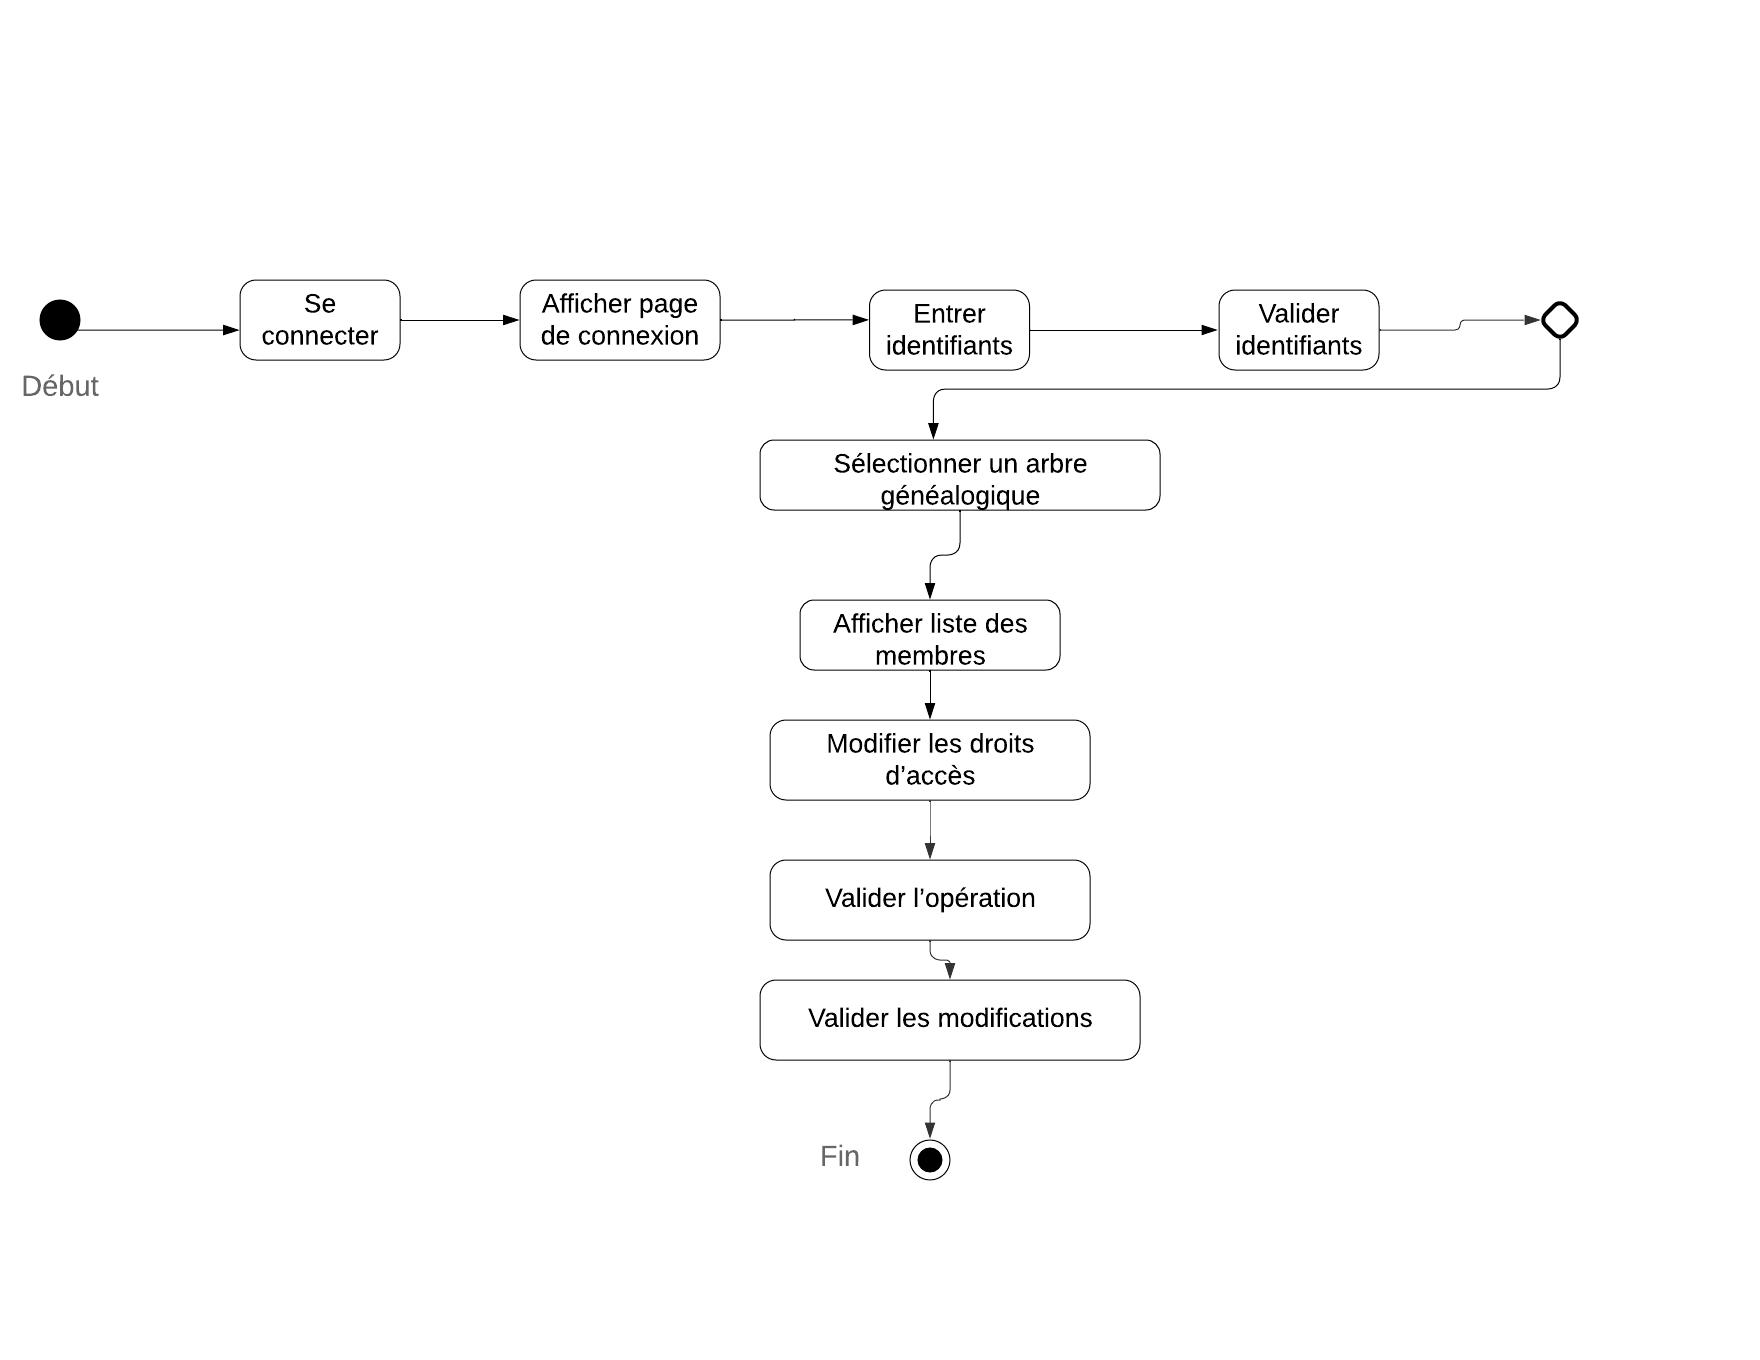
\includegraphics[width=1\textwidth]{figure/usecase2.png}
  \caption{Diagramme d'activité du cas d'utilisation accorder des droits d'accès}
\end{figure}


\subsection{Réalisations des cas d'utilisation}
Dans cette section, nous abordons la mise en œuvre concrète des cas
d’utilisation identifiés précédemment. À ce stade, nous traduisons les
interactions entre les acteurs et le système en fonctionnalités opérationnelles.
Nous détaillons également les règles de gestion spécifiques qui guident le
comportement du système lors de l’exécution de chaque cas d’utilisation. Enfin,
nous présentons le modèle du domaine sous forme d’un diagramme de classe du
système, offrant ainsi une vue structurée des entités et de leurs relations
au sein du système.
\subsubsection{Quelques règles de gestion}

Nous allons établir ici un ensemble de règles de gestion qui régissent le
comportement des fonctionnalités mises en œuvre. Ces règles définissent les
contraintes et les conditions d’exécution pour garantir la cohérence et la
fiabilité des opérations réalisées par le système.

\begin{itemize}
  \item \textbf{Règle de gestion 1 :} un membre ne peut pas modifier un arbre généalogique qui ne lui appartient pas.
  \item \textbf{Règle de gestion 2 :} un arbre généalogique privé ne peut être consulté que par ceux ayant des droits.
  \item \textbf{Règle de gestion 3 :} un arbre généalogique publique peut être consulté par tous les utilisateurs.
  \item \textbf{Règle de gestion 4 :} un arbre généalogique ne être supprimé que par un  membre ayant le droit d'adminitration.
  \item \textbf{Règle de gestion 5 :} un membre ne peut pas être ajouté deux fois à un arbre généalogique.
\end{itemize}

\subsubsection{Modèle du domaine (Diagramme de classe du système)}
Le diagramme de classe du système est une représentation visuelle des
entités principales du domaine et de leurs relations. Il offre une vue
d'ensemble de la structure du système, en mettant en évidence les différentes
classes d'objets, leurs attributs et leurs associations. Cette représentation
facilite la compréhension des concepts clés du domaine et guide la conception
de la solution logicielle.


% \newpage
\begin{figure}[H]
  \begin{tikzpicture}

    % Utilisateur class
    \umlclass{Utilisateur}{
      + id : String \\
      + nomUtilisateur : String \\
      + email : String \\
      + mdpHache : String \\
      + dateCreation : DateTime \\
      + dateModification : DateTime
    }{
      + creerUtilisateur() : void \\
      + mettreAJourUtilisateur(id) : void \\
      + supprimerUtilisateur() : void \\
      + authentifierUtilisateur(nom, mdp) : bool
    }

    % Session class
    \umlclass[x=0, y=-7]{Session}{
      + id : String \\
      + utilisateurId : String \\
      + dateExpiration : DateTime
    }{
      + creerSession(id) : void \\
      + terminerSession(id) : void
    }

    % AccesUtilisateur class
    \umlclass[x=9, y=-7]{AccesUtilisateur}{
      + id : String \\
      + niveau : NiveauAcces \\
      + utilisateurId : String \\
      + arbreId : String
    }{
      + attribuerAcces(id, ni) : void \\
      + mettreAJourAcces(id) : void \\
      + supprimerAcces(id) : void
    }

    % Arbre class
    \umlclass[x=9, y=-14]{Arbre}{
      + id : String \\
      + nom : String \\
      + type : TypeArbre
    }{
      + creerArbre() : void \\
      + mettreAJourArbre(id: String) : void \\
      + supprimerArbre(id: String) : void \\
      + ajouterMembre() : void \\
      + supprimerMembre(id: String) : void
    }

    % Membre class
    \umlclass[x=0, y=-13]{Membre}{
      + id : String \\
      + prenom : String \\
      + nom : String \\
      + dateNaissance : DateTime \\
      + lieuNaissance : String \\
      + genre : Genre \\
      + avatarURL : String \\
      + description : String \\
      + idPere : String \\
      + idMere : String
    }{
      + creerMembre() : void \\
      + mettreAJourMembre(id) : void \\
      + supprimerMembre(id) : void
    }

    % Enums
    \umlenum[x=9,]{NiveauAcces}{
      ADMIN \\
      EDITEUR \\
      LECTEUR
    }

    \umlenum[x=9, y=-19]{TypeArbre}{
      PUBLIC \\
      PRIVE
    }

    \umlenum[y=-20]{Genre}{
      M \\
      F
    }

    % Aggregations and Compositions
    \umluniaggreg[mult1=*, pos1=0.7, mult2=1, pos2=0.3]{Utilisateur}{Session}
    \umluniaggreg[mult1=*, pos1=0.7, mult2=1, pos2=0.3]{Utilisateur}{AccesUtilisateur}
    \umluniaggreg[mult1=*, pos1=0.7, mult2=1, pos2=0.3]{Arbre}{Membre}
    \umluniaggreg[mult1=*, pos1=0.7, mult2=1, pos2=0.3]{Arbre}{AccesUtilisateur}

    % Relationships
    \umluniassoc[mult1=1, pos1=0.7, mult2=1, pos2=0.3]{Session}{Utilisateur}
    \umluniassoc[mult1=1, pos1=0.7, mult2=1, pos2=0.3]{AccesUtilisateur}{Utilisateur}
    \umluniassoc[mult1=1, pos1=0.7, mult2=1, pos2=0.3]{AccesUtilisateur}{Arbre}
    \umluniassoc[mult1=1, pos1=0.7, mult2=1, pos2=0.3]{Membre}{Arbre}
    \umluniassoc[mult1=0..1, pos1=0.7, mult2=*, pos2=0.3]{Membre}{Membre}

    % Enum Relations
    \umluniassoc[mult1=1, pos1=0.7, mult2=*, pos2=0.3]{AccesUtilisateur}{NiveauAcces}
    \umluniassoc[mult1=1, pos1=0.7, mult2=*, pos2=0.3]{Arbre}{TypeArbre}
    \umluniassoc[mult1=1, pos1=0.7, mult2=*, pos2=0.3]{Membre}{Genre}

  \end{tikzpicture}
  \caption{Diagramme de classe du système mis à jour avec opérations}
\end{figure}




\subsubsection{Diagramme d'objet}
Un diagramme d’objet représente graphiquement les objets et leurs relations à
un moment donné. À l’inverse du diagramme de classe, qui décrit la structure
statique des classes et de leurs relations dans un système, le diagramme
d’objet illustre des instances spécifiques des classes (objets) et les liens
entre eux dans un contexte particulier. Il est utilisé pour visualiser l’état
d’un système à un instant précis, facilitant la compréhension des interactions
dynamiques et des configurations temporaires des objets.

\begin{figure}[H]
    \centering
    \begin{tikzpicture}[
        object/.style={rectangle, draw, text width=6cm, minimum height=1cm, align=left, font=\ttfamily},
        attribute/.style={text width=7cm, align=left, font=\ttfamily}
    ]

        % Object instances with separation bar
        \node[object] (utilisateur1) {
            \textbf{Utilisateur: utilisateur1} \\
            \rule{\linewidth}{0.4pt} \\  % Horizontal line
            \underline{id} = "u1234" \\
            \underline{nomUtilisateur} = "jdoe" \\
            \underline{email} = "jdoe@example.com" \\
            \underline{MdpHaché} = "******" \\
            \underline{DateCreation} = "2022-01-01" \\
            \underline{DateModifier} = "2022-02-01"
        };

        \node[object, below=of utilisateur1] (session1) {
            \textbf{Session: session1} \\
            \rule{\linewidth}{0.4pt} \\  % Horizontal line
            \underline{id} = "s1234" \\
            \underline{userId} = "u1234" \\
            \underline{expiresAt} = "2022-02-01"
        };

        \node[object, right=of utilisateur1] (acces1) {
            \textbf{AccèsUtilisateur: acces1} \\
            \rule{\linewidth}{0.4pt} \\  % Horizontal line
            \underline{id} = "a1234" \\
            \underline{niveau} = "admin" \\
            \underline{userId} = "u1234" \\
            \underline{treeId} = "t1234"
        };

        \node[object, below=of acces1] (arbre1) {
            \textbf{Arbre: arbre1} \\
            \rule{\linewidth}{0.4pt} \\  % Horizontal line
            \underline{id} = "t1234" \\
            \underline{name} = "Doe Family Tree" \\
            \underline{type} = "privé"
        };

        \node[object, below=of session1] (member1) {
            \textbf{Membre: member1} \\
            \rule{\linewidth}{0.4pt} \\  % Horizontal line
            \underline{id} = "m1234" \\
            \underline{prenom} = "Jane" \\
            \underline{nom} = "Doe" \\
            \underline{dateNaissance} = "1990-01-01" \\
            \underline{lieuNaissance} = "Paris" \\
            \underline{genre} = "féminin" \\
            \underline{avatarURL} = "http://example.com/jane.jpg" \\
            \underline{description} = "Daughter of John Doe" \\
            \underline{idPere} = "m1235" \\
            \underline{idMere} = "m1236"
        };

        % Relationships
        \draw[->] (utilisateur1) -- (session1);
        \draw[->] (utilisateur1) -- (acces1);
        \draw[->] (acces1) -- (arbre1);
        \draw[->] (arbre1) -- (member1);

    \end{tikzpicture}
    \caption{Diagramme d'objet du système}
\end{figure}


\newpage
\subsection{Conception architecturale}
La conception architecturale est une étape importante du développement logiciel
qui vise à définir la structure globale d’un système et de ses composants
principaux. Elle comprend l’organisation des modules, la communication entre
eux et les contraintes techniques à respecter. Cette phase permet de créer une
base solide pour le développement, afin d’assurer que les exigences
fonctionnelles et non fonctionnelles seront satisfaites. La conception
architecturale se décline en plusieurs sous-sections, notamment l’architecture
logicielle et l’architecture globale de la solution.

\subsubsection{Architecture logicielle}
L’architecture logicielle décrit la structure organisationnelle d’un système
logiciel, y compris ses modules, leurs responsabilités et les interactions
entre eux. Elle vise à garantir la cohérence, la performance, la maintenabilité
et la scalabilité du système. L’architecture logicielle est un guide pour les
développeurs qui permet d’aligner les décisions techniques avec les objectifs
métier et les contraintes du projet.

Pour notre projet, nous avons opté pour une architecture basée sur plusieurs
projets dans un seul référentiel (Monorepo). Cette architecture permet de centraliser
le code des applications Android, iOS, et Web, ainsi que les composants partagés et le serveur backend.

\subsection*{Structure du Répertoire}

\paragraph{Racine du Projet}
\begin{itemize}
    \item \texttt{.env} : Fichier de configuration des variables d'environnement.
    \item \texttt{package.json} : Dépendances et scripts du projet.
    \item \texttt{tsconfig.json} : Configuration de TypeScript.
    \item \texttt{next.config.js} : Configuration de Next.js.
    \item \texttt{capacitor.config.ts} : Configuration de Capacitor.
\end{itemize}

\paragraph{android}
\begin{itemize}
    \item Contient le code et la configuration de l'application Android utilisant Capacitor.
\end{itemize}

\paragraph{ios}
\begin{itemize}
    \item Contient le code et la configuration de l'application iOS utilisant Capacitor.
\end{itemize}

\paragraph{out}
\begin{itemize}
    \item Contient les exportations statiques de l'application Web Next.js.
\end{itemize}

\paragraph{src}
\begin{itemize}
    \item \texttt{actions} : Actions server Next.js.
    \item \texttt{app} : Code principal de l'application Next.js.
    \item \texttt{components} : Composants React réutilisables.
    \item \texttt{lib} : Bibliothèques et fonctions utilitaires.
    \item \texttt{server} : Code backend, incluant les routes API et la configuration de la base de données.
    \item \texttt{styles} : Fichiers de styles.
    \item \texttt{trpc} : Configuration et handlers de tRPC.
    \item \texttt{types} : Types et interfaces TypeScript.
\end{itemize}

\subsection*{Interaction entre les Parties}

\begin{itemize}
    \item \textbf{Android et iOS} : Utilisent Capacitor pour intégrer des
      fonctionnalités Web dans les applications mobiles. Ils partagent du code
      et des composants avec l'application Web.
    \item \textbf{Web (Next.js)} : L'application principale qui utilise React
      pour le frontend et tRPC pour les appels API.
    \item \textbf{Server} : Fournit les API et gère les interactions avec la
      base de données. Partagé entre les applications Web et mobiles pour
      assurer la cohérence des données.
    \item \textbf{Components et Lib} : Répertoires partagés contenant les
      composants réutilisables et les fonctions utilitaires, facilitant la
      maintenance et la réutilisation du code.
\end{itemize}

Cette structure Monorepo centralisée permet une gestion cohérente et efficace
des différents aspects de l'application, en simplifiant le développement et la maintenance.

\begin{figure}[H]
  \centering
  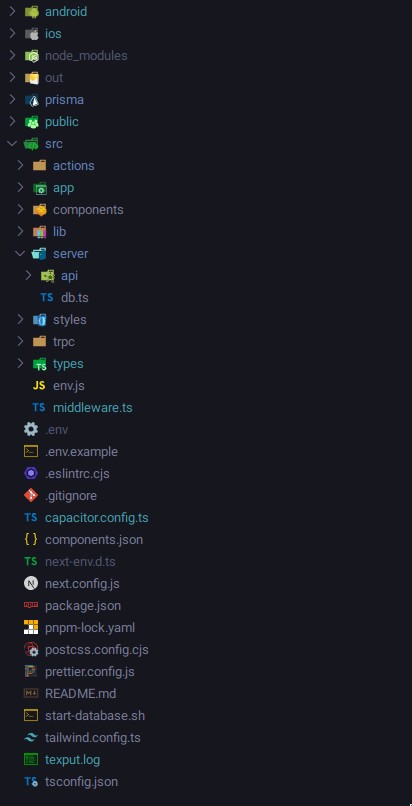
\includegraphics[width=0.5\textwidth]{figure/archi.png}
  \caption{Architecture du logiciel sous VSCodium}
\end{figure}

\subsubsection{Architecture globale de la solution (Diagramme de déploiement)}
L’architecture globale de la solution est souvent illustrée par un diagramme de
déploiement qui montre la configuration physique des composants logiciels sur
le matériel. Ce diagramme détaille comment les éléments logiciels sont
distribués à travers différents nœuds de réseau, tels que serveurs, bases de
données, et terminaux utilisateurs. Il aide à comprendre les aspects de
performance, de sécurité et de scalabilité de la solution, en montrant comment
les composants interagissent dans un environnement réel.

Dans notre cas, la plateforme pour la création collaborative et le partage
d’arbres généalogiques sont basés sur une architecture distribuée qui
comprend plusieurs composants clés.

Une architecture distribuée  désigne un système d'information ou un réseau pour
lequel l'ensemble des ressources disponibles ne se trouvent pas au même endroit
ou sur la même machine (Wikipédia).

\begin{figure}[H]
  \centering
  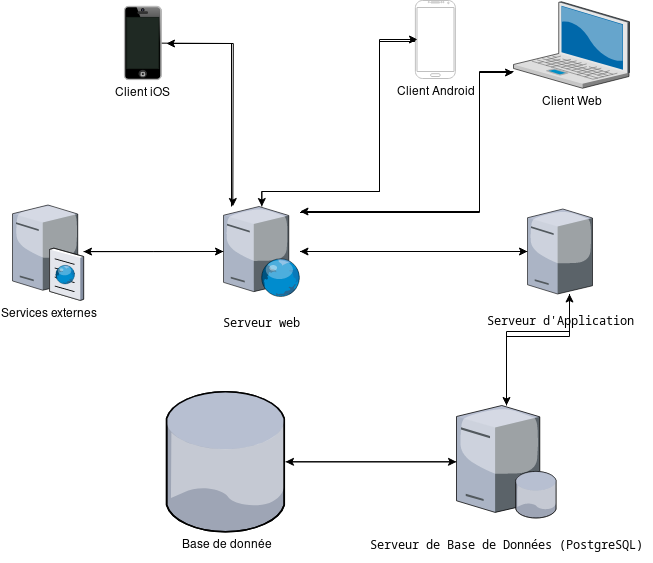
\includegraphics[width=0.5\textwidth]{figure/schema.png}
  \caption{Illustration d'une architecture distribuée}
\end{figure}

\begin{itemize}
  \item \textbf{ Serveur Web :} Héberge l'application Next.js pour le rendu
    côté serveur (SSR) et le serveur API. Utilise Node.js pour exécuter le
    code JavaScript côté serveur.

  \item \textbf{Serveur d'application :} utilise Node.js et Next.js pour
    le rendu côté serveur et la génération de pages statiques.

  \item \textbf{Serveur de bases de données :} utilise PostgreSQL comme SGBD
    pour stocker les données relatives aux utilisateurs, aux arbres
    généalogiques et aux collaborations.

  \item \textbf{ Terminal utilisateur :} comprend les navigateurs Web pour
    accéder à l’application web Next.js et les applications mobiles Capacitor
    pour l’accès mobile.

  \item \textbf{Services externes :} intègre éventuellement des services
    externes pour des fonctionnalités supplémentaires, telles que
    le stockage de fichiers et les
    services de messagerie.

\end{itemize}

Voici un diagramme de déploiement illustrant cette architecture :

\begin{figure}[H]
  \centering
  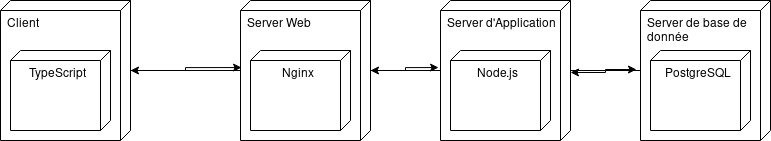
\includegraphics[width=1\textwidth]{figure/deployemnt.drawio(1).png}
  \caption{Diagramme de déploiement logique}
\end{figure}

\textbf{Avantages de cette architecture }

\begin{itemize}
  \item \textbf{Scalabilité:} les composants peuvent être mis à l’échelle
    indépendamment en fonction de la demande.

  \item \textbf{Sécurité :} la séparation des préoccupations permet
    d’améliorer la sécurité, notamment en isolant la base de données
    du reste de l’application.

  \item \textbf{Performance :} l'utilisation du rendu côté serveur et de la
    génération de pages statiques améliore la vitesse de chargement des
    pages et l’expérience utilisateur.

  \item \textbf{Maintenabilité :} l’architecture distribuée permet d’intégrer
    de nouveaux services et de mettre à jour les composants sans affecter
    l’ensemble du système.

\end{itemize}
